\section{2020 年 9 月 22 日答疑记录}

\begin{example}
  已知二次函数 $y= x^2-2ax+1$, 当 $2<x<3$ 时, 函数值 $y$ 随 $x$ 的增大而减小, 求实数 $a$ 的取值范围.
\end{example}
\begin{solution}
  $y= x^2-2ax+1$ 的图象为开口向上的抛物线, 对称轴为 $x= -\dfrac{-2a}{2\cdot 1}= a$. 由题意, 当 $2<x<3$ 时, $x$ 在对称轴的左侧, 所以 $3\leqslant a$, 即 $a\in [3,+\infty)$.
\end{solution}
\begin{remark}
  (1) 二次函数 $y= Ax^2+Bx+C$ ($A\neq 0$) 的单调性可以通过观察其图象 (抛物线) 的开口方向 (由 $A$ 的正负号决定) 和对称轴 $x= -\dfrac{B}{2A}$ 的位置得出.
  
  (2) 写二次函数的对称轴时, 只需按照公式的格式写出对应的式子 (见解答第 1 行), 无需明确地写出公式. 如果对称轴容易口算, 也可直接写出, 如本题可直接写 ``对称轴为 $x= a$''.
\end{remark}

\begin{example}
  对二次函数 $y=x^2-2x+2$, 当 $t\leqslant x\leqslant t+1$ 时, 求函数值 $y$ 的最大值与最小值.
\end{example}
\begin{solution}
  $y=x^2-2x+2= (x-1)^2+1$ 的图象为开口向上的抛物线, 对称轴为 $x=1$. 下面考虑定义域与对称轴的相对位置, 再确定对应函数值的最大 (小) 值.
  
  (1) 若 $t+1\leqslant 1$ 即 $t\leqslant 0$, 则当 $x=t$ 时, $y=t^2-2t+2$ 为最大值; 当 $x=t+1$ 时, $y=t^2+1$ 为最小值.
  
  (2) 若 $\dfrac{t+(t+1)}2\leqslant 1< t+1$ 即 $0<t\leqslant \dfrac12$, 则当 $x=t$ 时, $y=t^2-2t+2$ 为最大值; 当 $x=1$ 时, $y=1$ 为最小值.
  
  (3) 若 $t\leqslant 1< \dfrac{t+(t+1)}2$ 即 $\dfrac12< t\leqslant 1$, 则当 $x=t+1$ 时, $y=t^2+1$ 为最大值; 当 $x=1$ 时, $y=1$ 为最小值.
  
  (4) 若 $1< t$ 即 $t> 1$, 则当 $x=t+1$ 时, $y=t^2+1$ 为最大值; 当 $x=t$ 时, $y=t^2-2t+2$ 为最小值.
  
  下图为情形 (1) (2) 对应的示意图:
  
  \begin{center}
  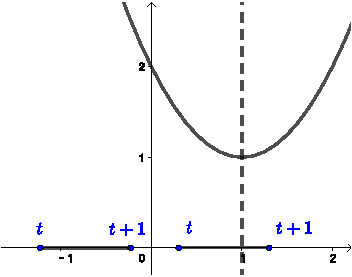
\includegraphics{2020-1007-1710-crop}
  \end{center}
\end{solution}
\begin{remark}
  (1) 除了直接用公式, 二次函数的对称轴也可以通过配方得出, 如解答第 1 行.
  
  (2) 求二次函数部分图像的最大 (小) 值, 需要考虑定义域与对称轴的相对位置, 共四种: 对称轴在定义域右侧 (情形 (1)); 对称轴在定义域内偏右 (情形 (2)); 对称轴在定义域内偏左 (情形 (3)); 对称轴在定义域左侧 (情形 (4)), 其中情形 (2) (3) 均需考虑定义域的中点.
  
  (3) 分类讨论时需注意 ``不重不漏'', 且应明确写出参数的范围 (如各种情形的第 1 行).
\end{remark}